% couette-flow-3D.tex

\newpage
\section{Couette Flow: 3D}
\label{couette-flow-3D}
%
The three dimensional couette flow is also studied, the front and side view are shown in
Figure~\ref{couette3-frontside-fig}, respectively. Since we are going to monitor the velocity profile along
$z$ direction, there is the high resolution compared to the grid at $x$ and $y$ direction. The top surface
is set as Moving Wall boundary condition, while the BOTTOM surface Adiabatic wall. The Slip Wall boundary
conditions were set both the the WEST and EAST surface, the NORTH and SOUTH surfaces are connected
with the fuction of \texttt{connect\_blocks\_3D}, since the NORTH and SOUTH are not connected
physically, please note that the boolean parameter of \texttt{check\_corner\_locations} should be
\textbf{False}, or it would connect incorrectly.

\begin{figure}[htbp]
\begin{center}
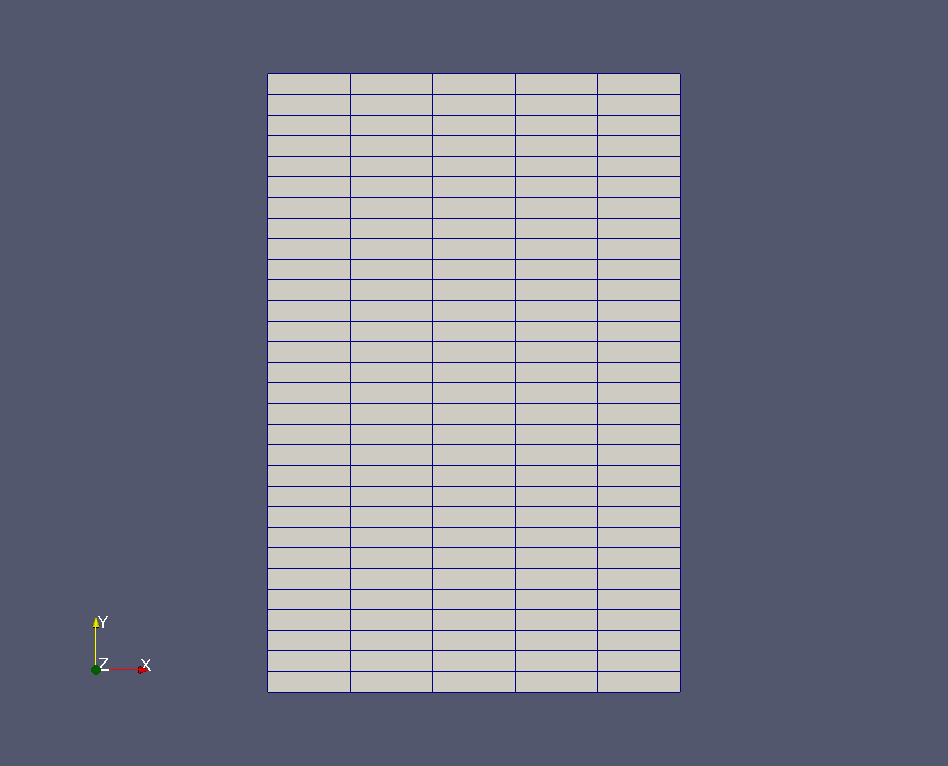
\includegraphics[width=0.45\textwidth]{../3D/couette-flow/front-view.png}
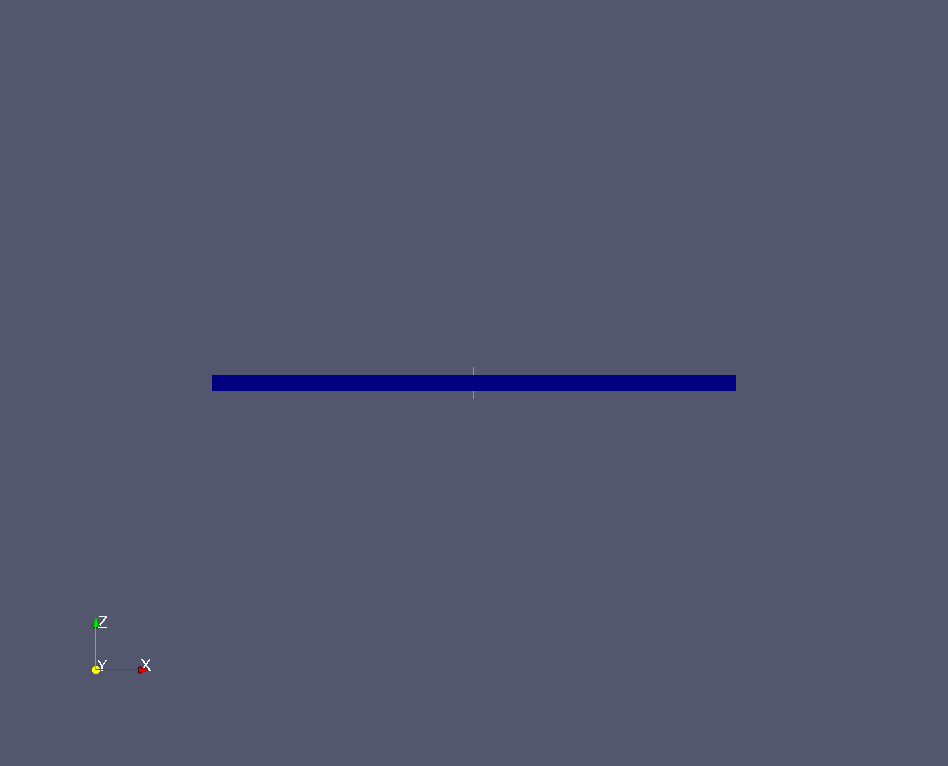
\includegraphics[width=0.45\textwidth]{../3D/couette-flow/side-view.png}
\end{center}
\caption{Front and side view of 3D couette flow.}
   \label{couette3-frontside-fig}
\end{figure}


\begin{figure}[htbp]
\begin{center}
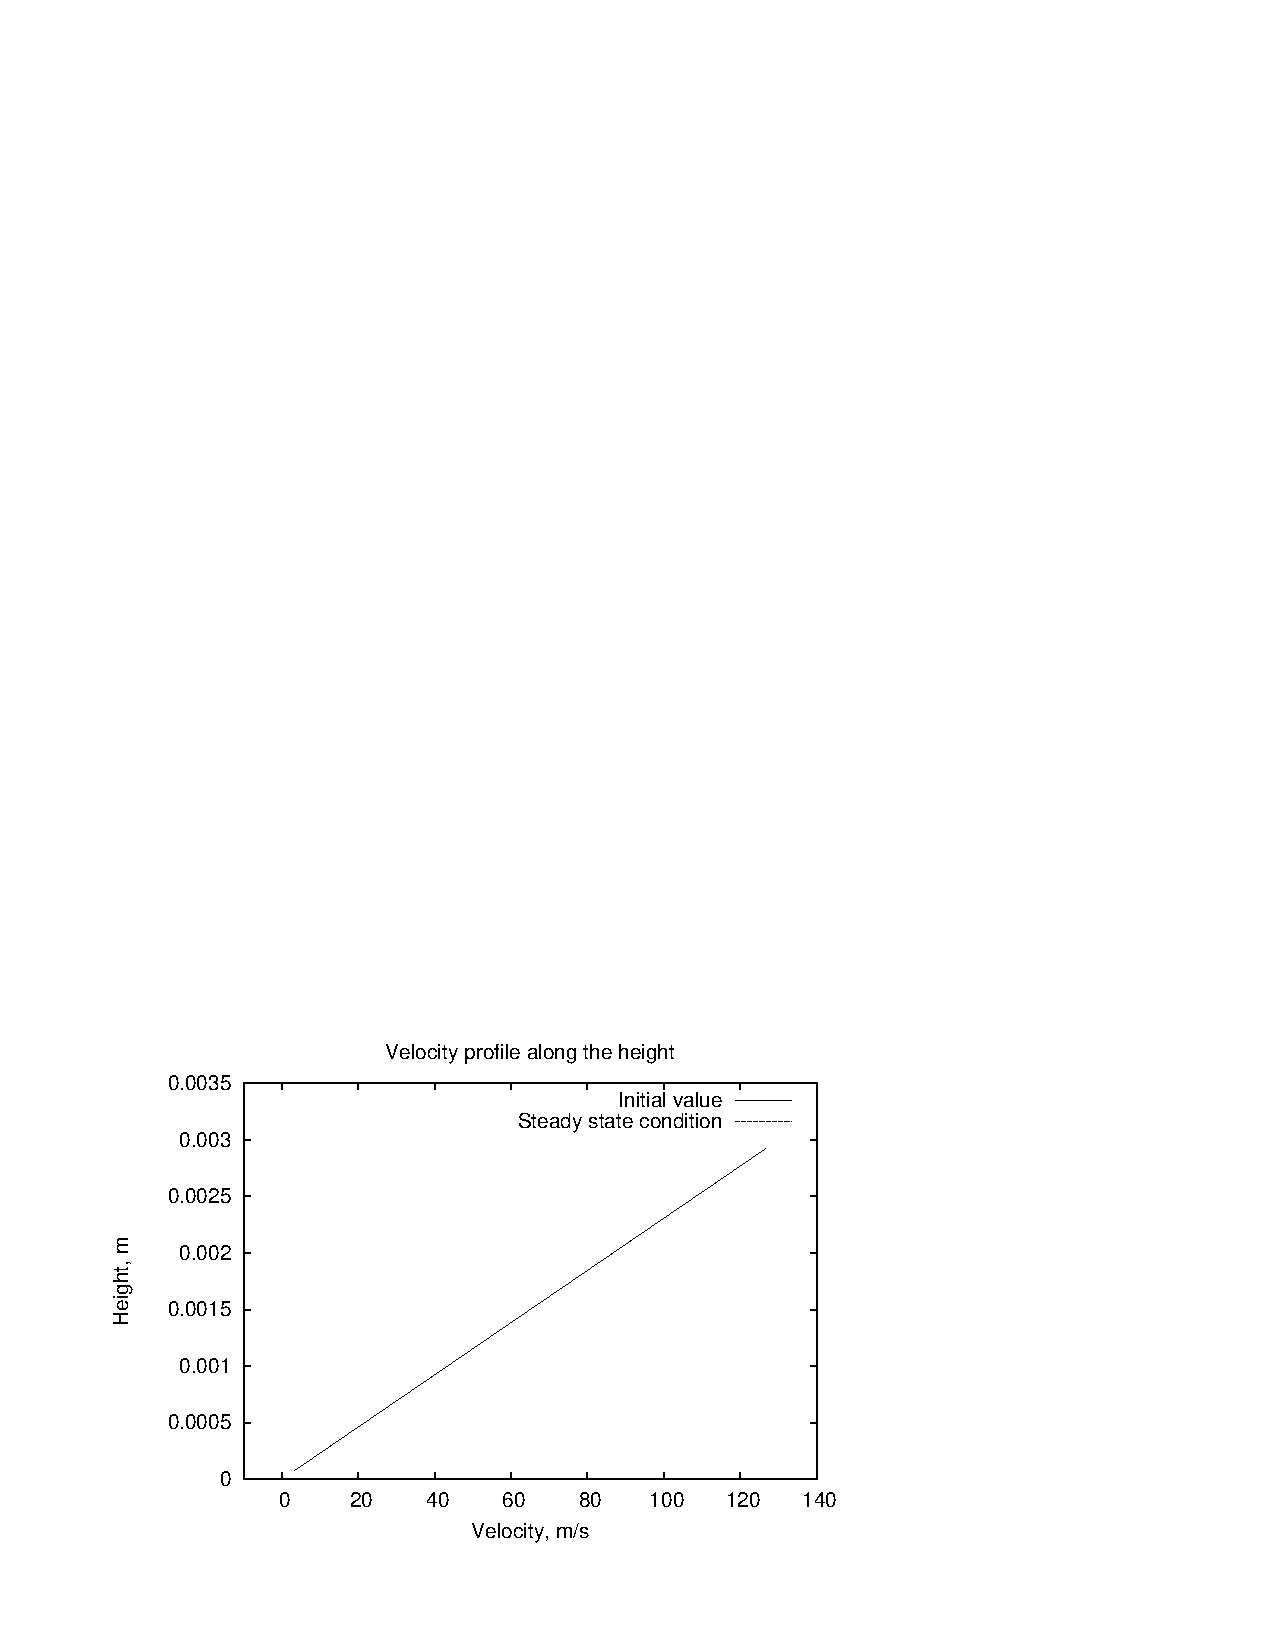
\includegraphics[width=0.45\textwidth,viewport=39 52 414 298,clip=true]{../3D/couette-flow/c_3D_linear.pdf}
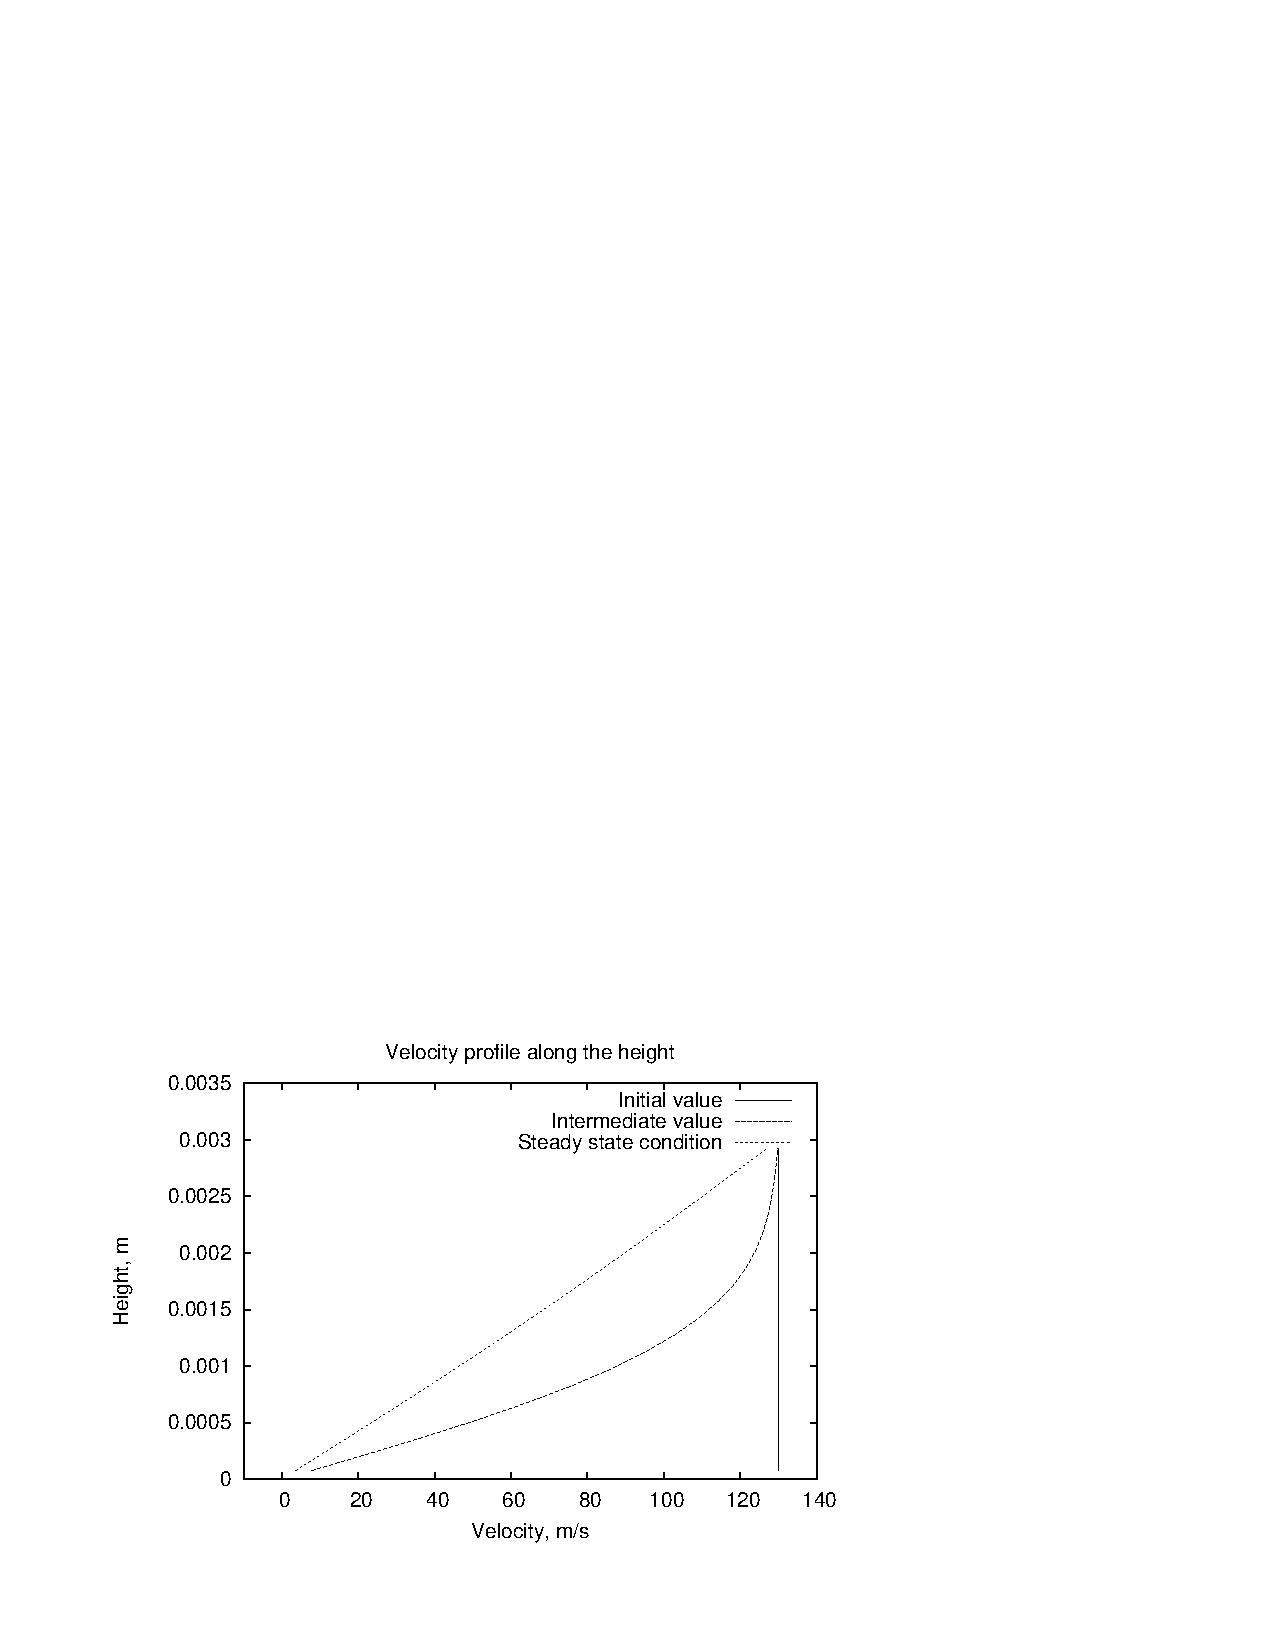
\includegraphics[width=0.45\textwidth,viewport=39 52 414 298,clip=true]{../3D/couette-flow/c_3D_uniform.pdf}
\end{center}
\caption{Velocity profile along the height: linear and uniform velocity.}
   \label{couette3-linearuniform-fig}
\end{figure}

\medskip
It should be noted that the initial value would have a high effect on the computation time 
for this test case. The velocity profile along the height with differect initial values are 
shown in Figure~\ref{couette3-linearuniform-fig}, respectively. We can see that it would cost too much time for
uniform velocity compared to linear velocity.

\newpage
\subsection{Input script (.py)}
\topbar
\lstinputlisting[language={}]{../3D/couette-flow/couette.py}
\bottombar


\subsection{Shell scripts}
\label{couette-flow-3D-sh-files}
\topbar
\lstinputlisting[language={}]{../2D/couette-flow/couette.sh}
\bottombar

\subsection{Notes}
\begin{itemize}
\item None
\end{itemize}


